\chapter{Testing and results}
\label{chap:results}

To prove that system is working a test was conducted at the Ubiquitous Computing Laboratory at \ac{HTWG}. Four rows of six \ac{FSR} sensors were placed on the pressure-disks. Sensors were placed in shoulder and lower torso area where it's easiest to detect vital signs. Two nodes and Intel Edison were attached to the bottom of the bed frame and connected to the sensors. To power the whole system an external 2.500mAh battery was used. Assembled system can be seen in Figure \ref{fig:bed_sensors}. Previously used system required 2 nodes, 10 hand soldered boards and over 35 wires to function while the new one was set up in less than 15 minutes when all sensors were installed on the pressure-disk blades.

\begin{figure}[h]
  \begin{center}
    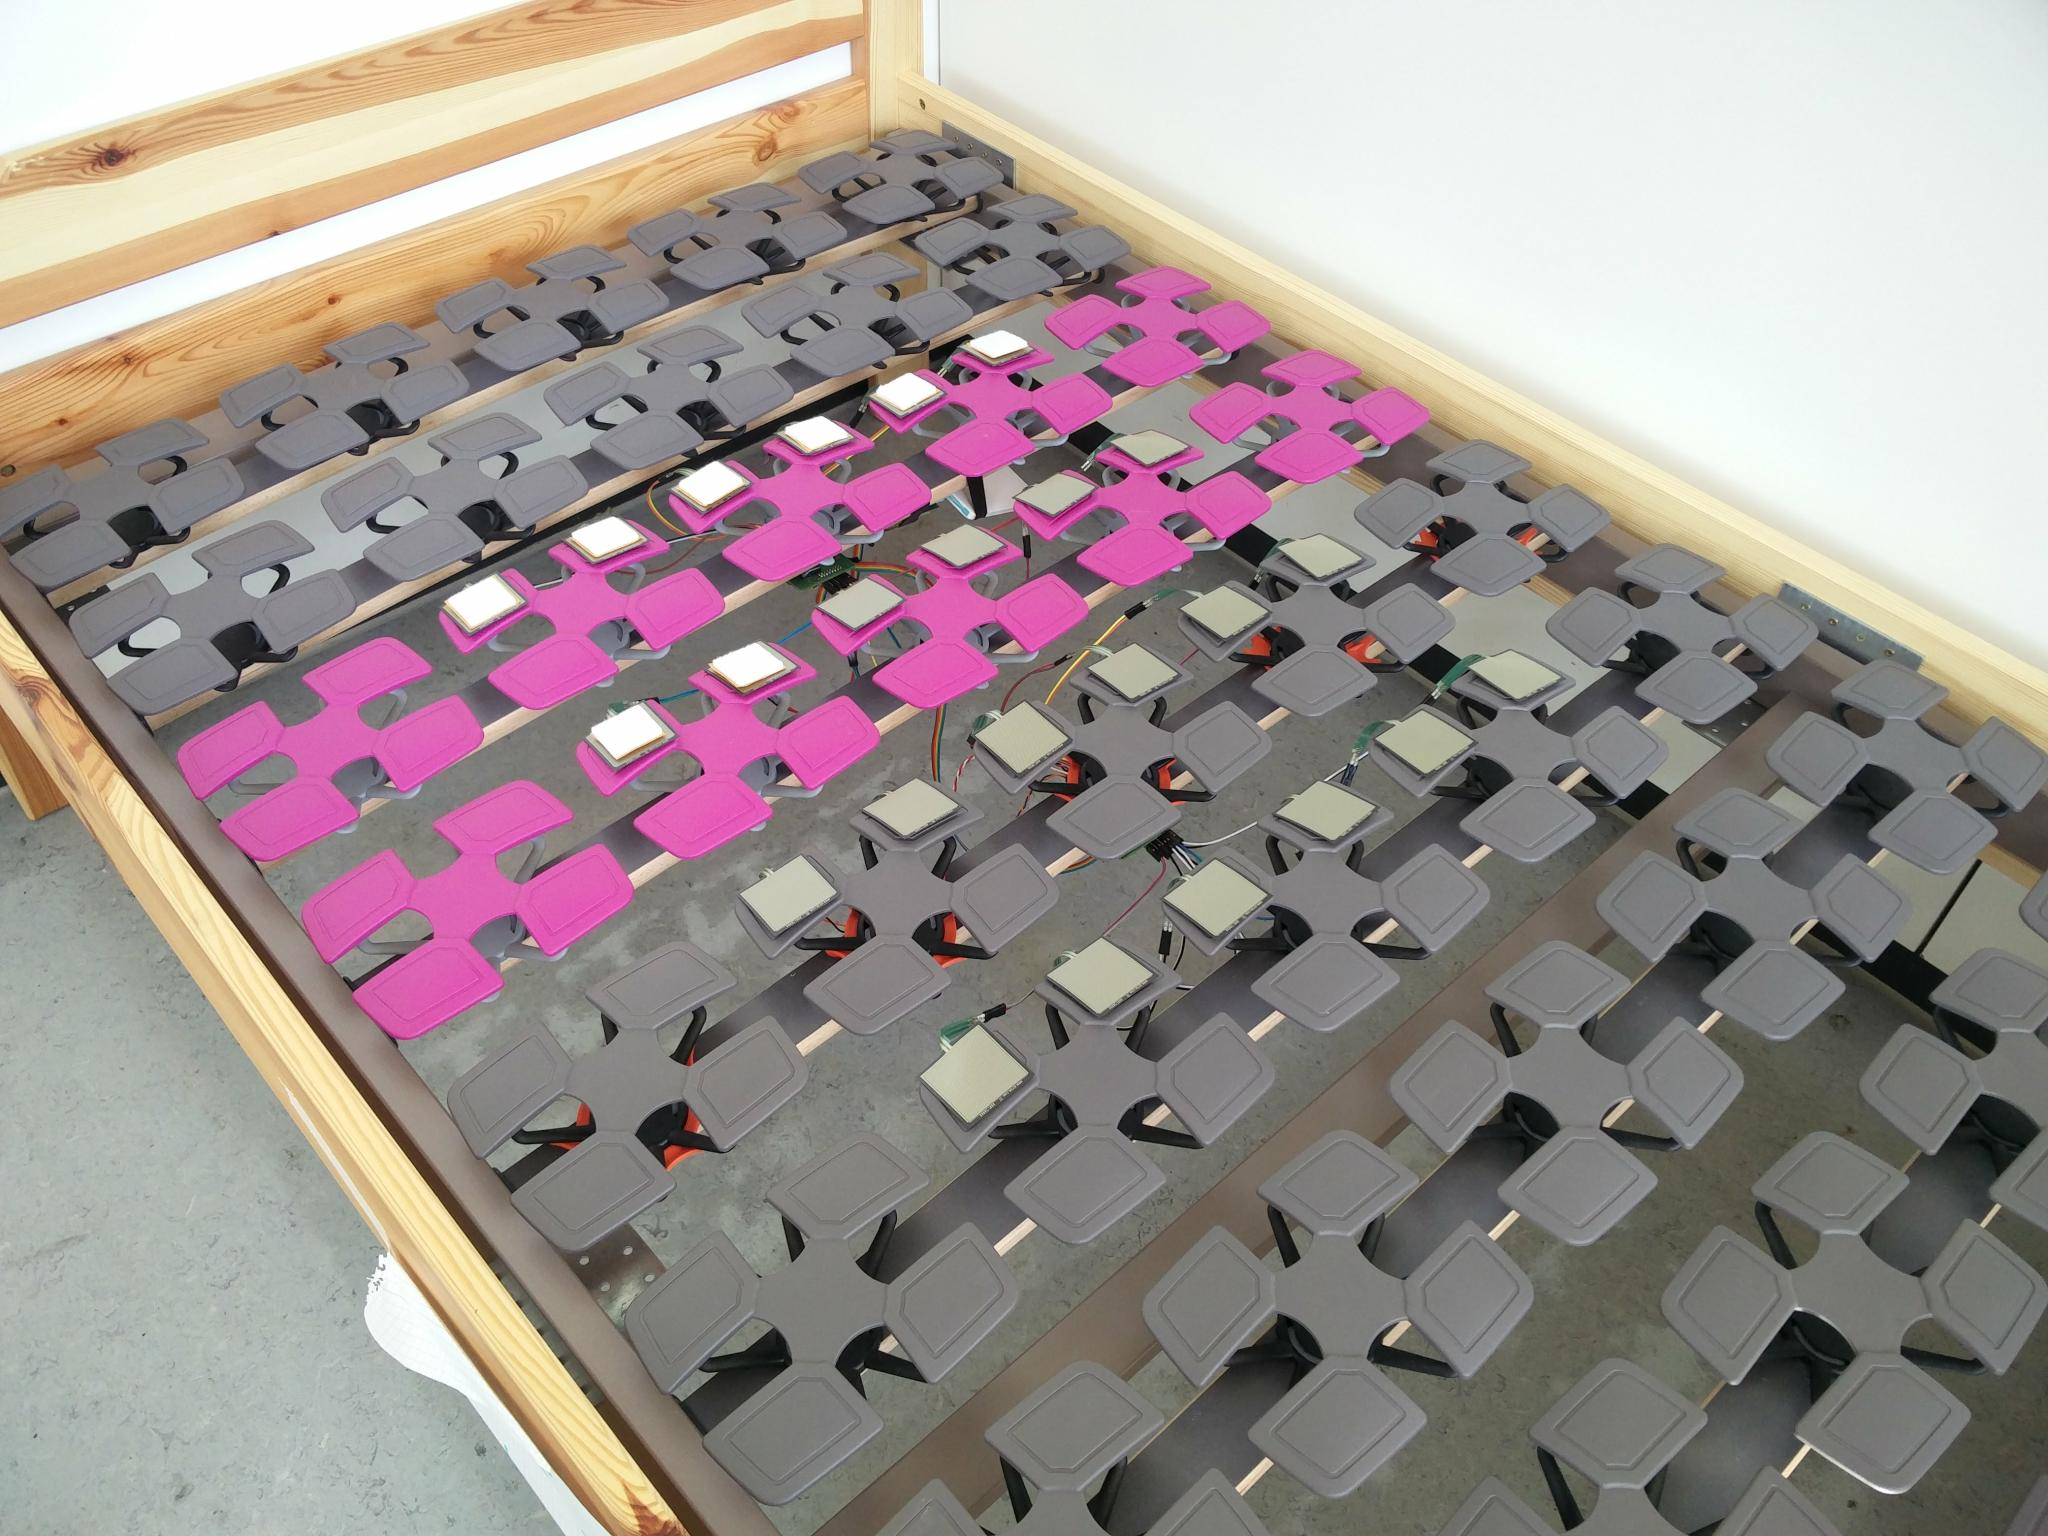
\includegraphics[width=0.40\linewidth]{6-bed_sensors_top.jpg}
    \vspace{0.5cm}
    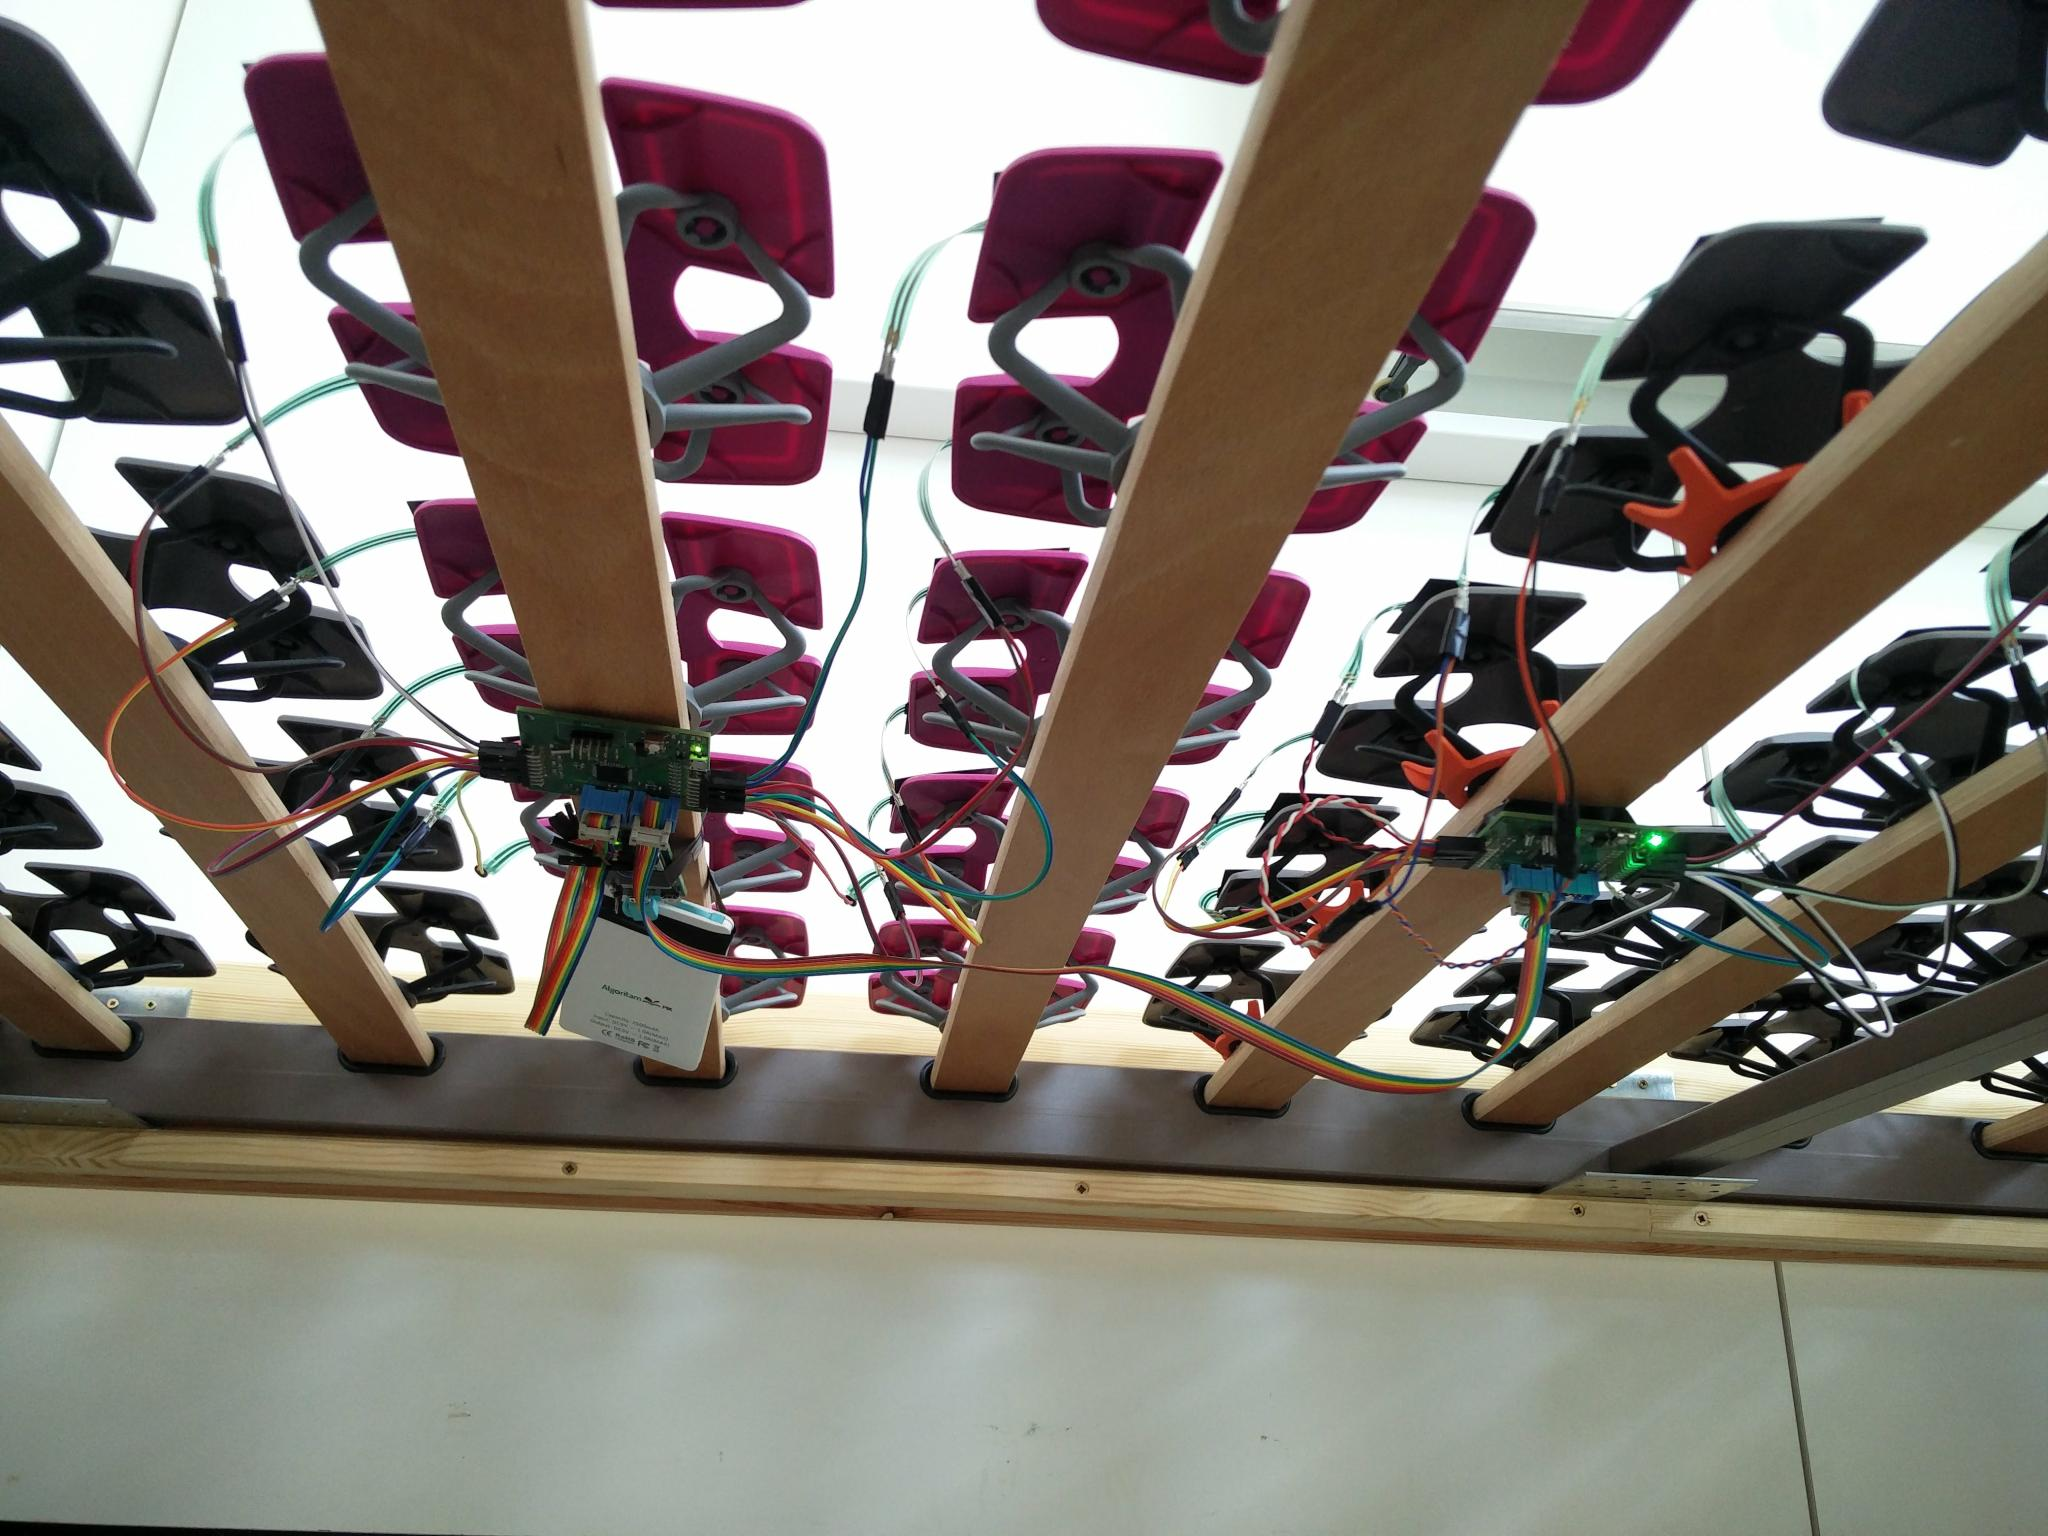
\includegraphics[width=0.40\linewidth]{6-bed_sensors_bottom.jpg}
  \end{center}
  \caption{Sensors and nodes installed into the bed.}
  \label{fig:bed_sensors}
\end{figure}

First test was conducted to see if all of the sensors work. Sensors were excited and results were tracked in real time using laptop connected to the same wireless network as an endpoint. It was observed that sensors 3 and 6 were not reacting to the applied pressure. After reinsertion of wires, sensor number 6 started working while it was found that the cause of sensor 3 malfunction was \ac{ADC} pin unresponsiveness. This issue was fixed by connecting another pin to the sensor but this remains to be fixed on the \ac{PCB}.

\begin{figure}[h]
  \begin{center}
    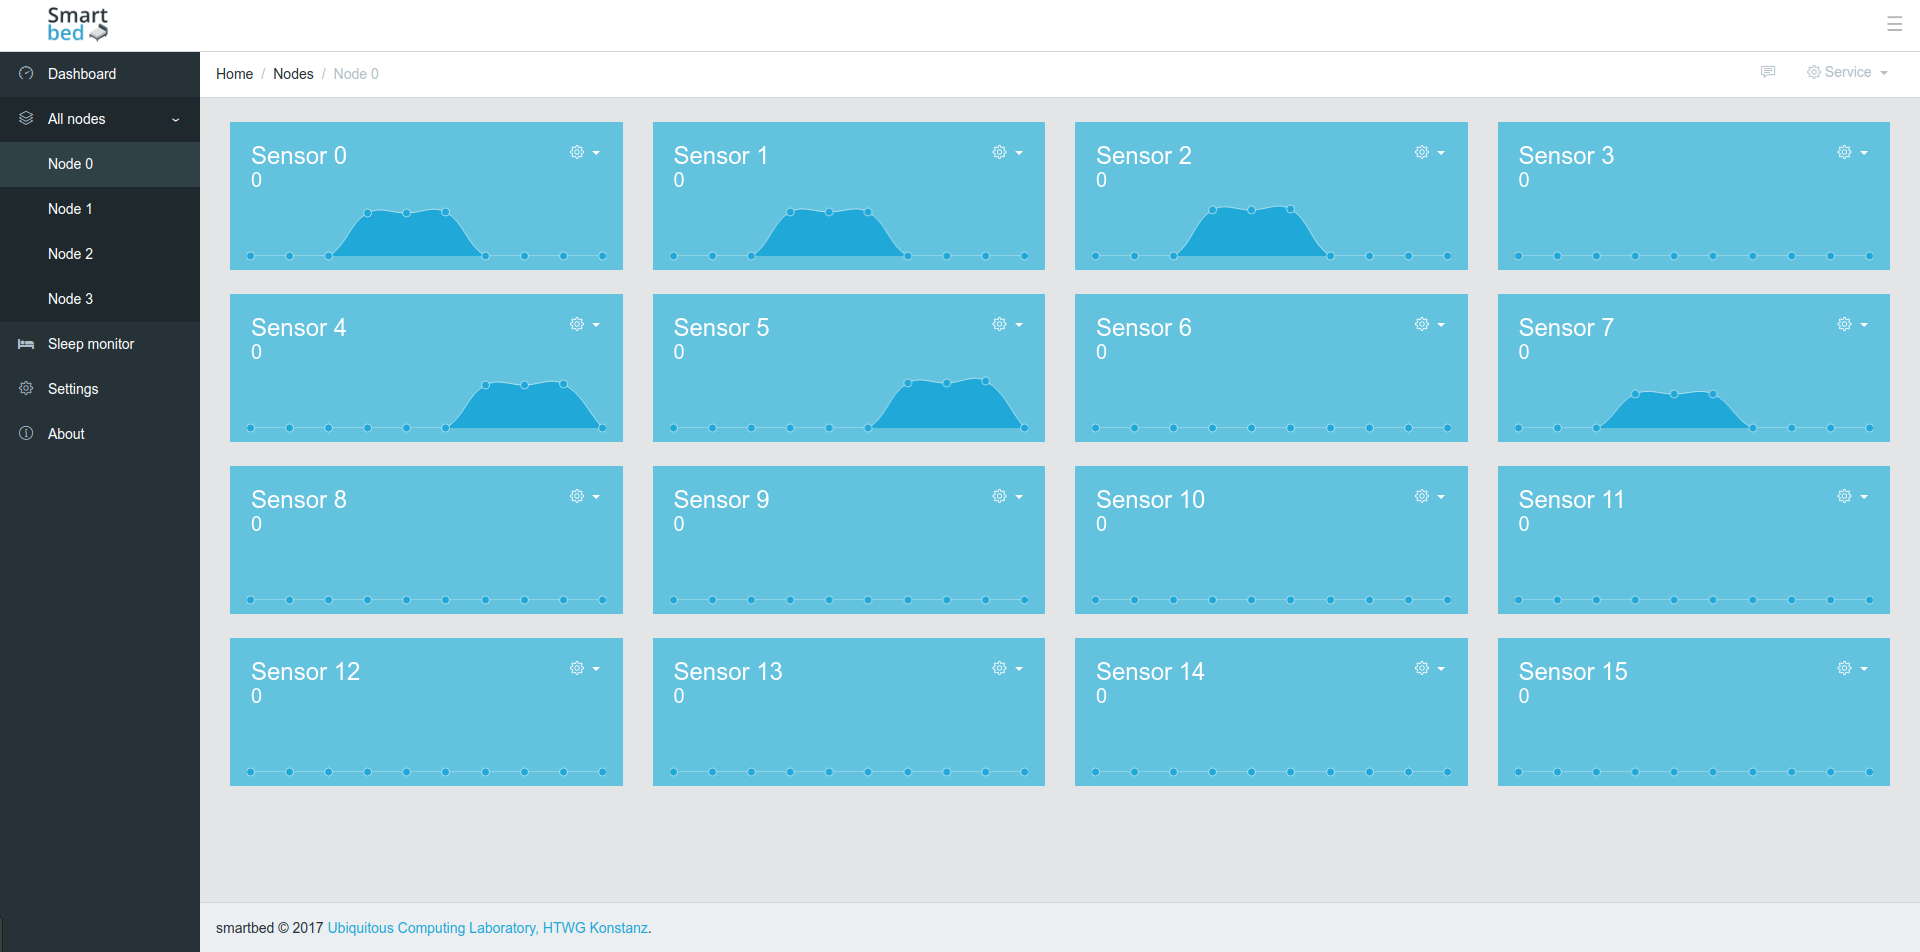
\includegraphics[width=0.75\linewidth]{6-testing.png}
  \end{center}
  \caption{Testing of the responsiveness and sensitivity.}
  \label{fig:testing}
\end{figure}

In the next phase, a mattress was placed onto the bed. In this position, a pressure detected by the sensors was lower than threshold set in the firmware so they were registering 0. A subject lied on the bed and rested in log position for 2 minutes after which he changed position to supine and rested for further 4 minutes. After that, data was exported to the CSV file and analysed. Charts found in Figure \ref{fig:node_1} and Figure \ref{fig:node_2} represent plotted sensor data on both nodes.

\begin{figure}[h]
  \begin{center}
    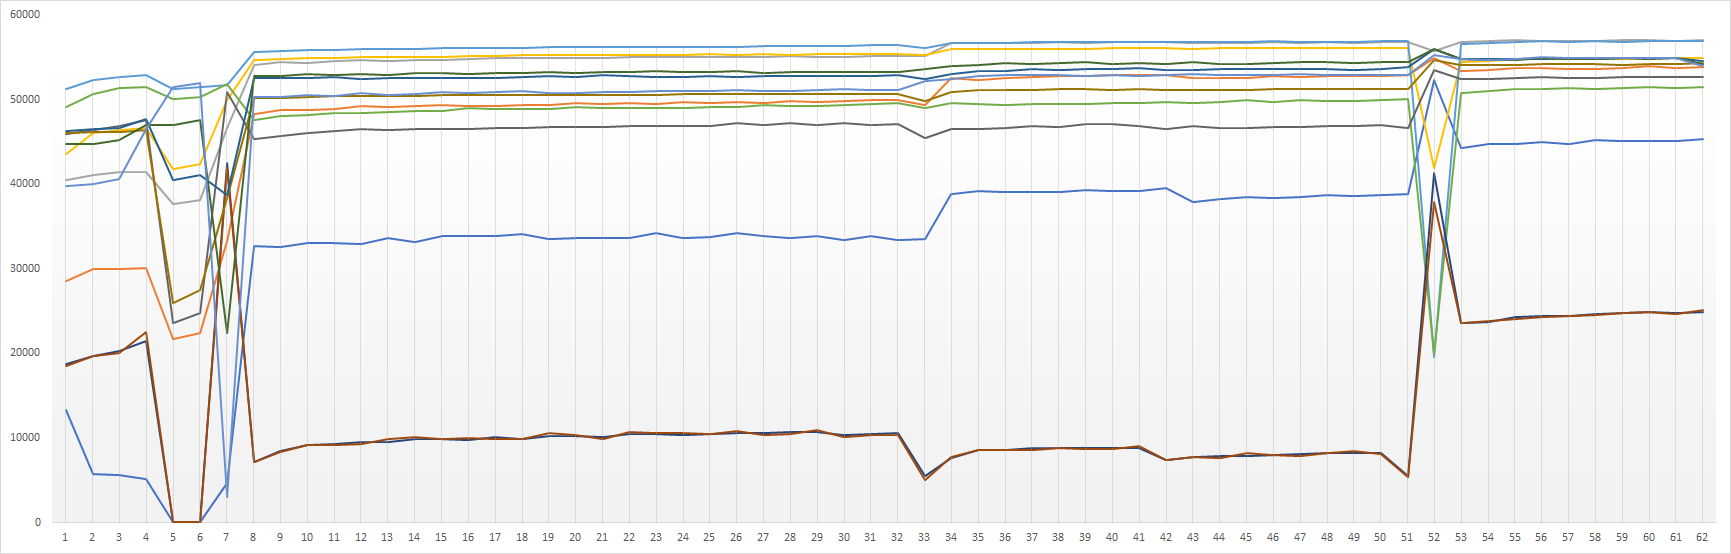
\includegraphics[width=\linewidth]{6-node_1.png}
  \end{center}
  \caption{Pressure measured on sensors in shoulder area.}
  \label{fig:node_1}
\end{figure}

When subject sat on the bed, sensors were excited with the peak value reaching 57118 while saturation values is 65535. Average value during the test for all of the sensors was 44565 which is 68\% of maximum value. While subject was still, values for each sensor were constantly fluctuating with an average deviation of 284 points. This means that 9-bit resolution for vital sign recognition was achieved. 

\begin{figure}[h]
  \begin{center}
    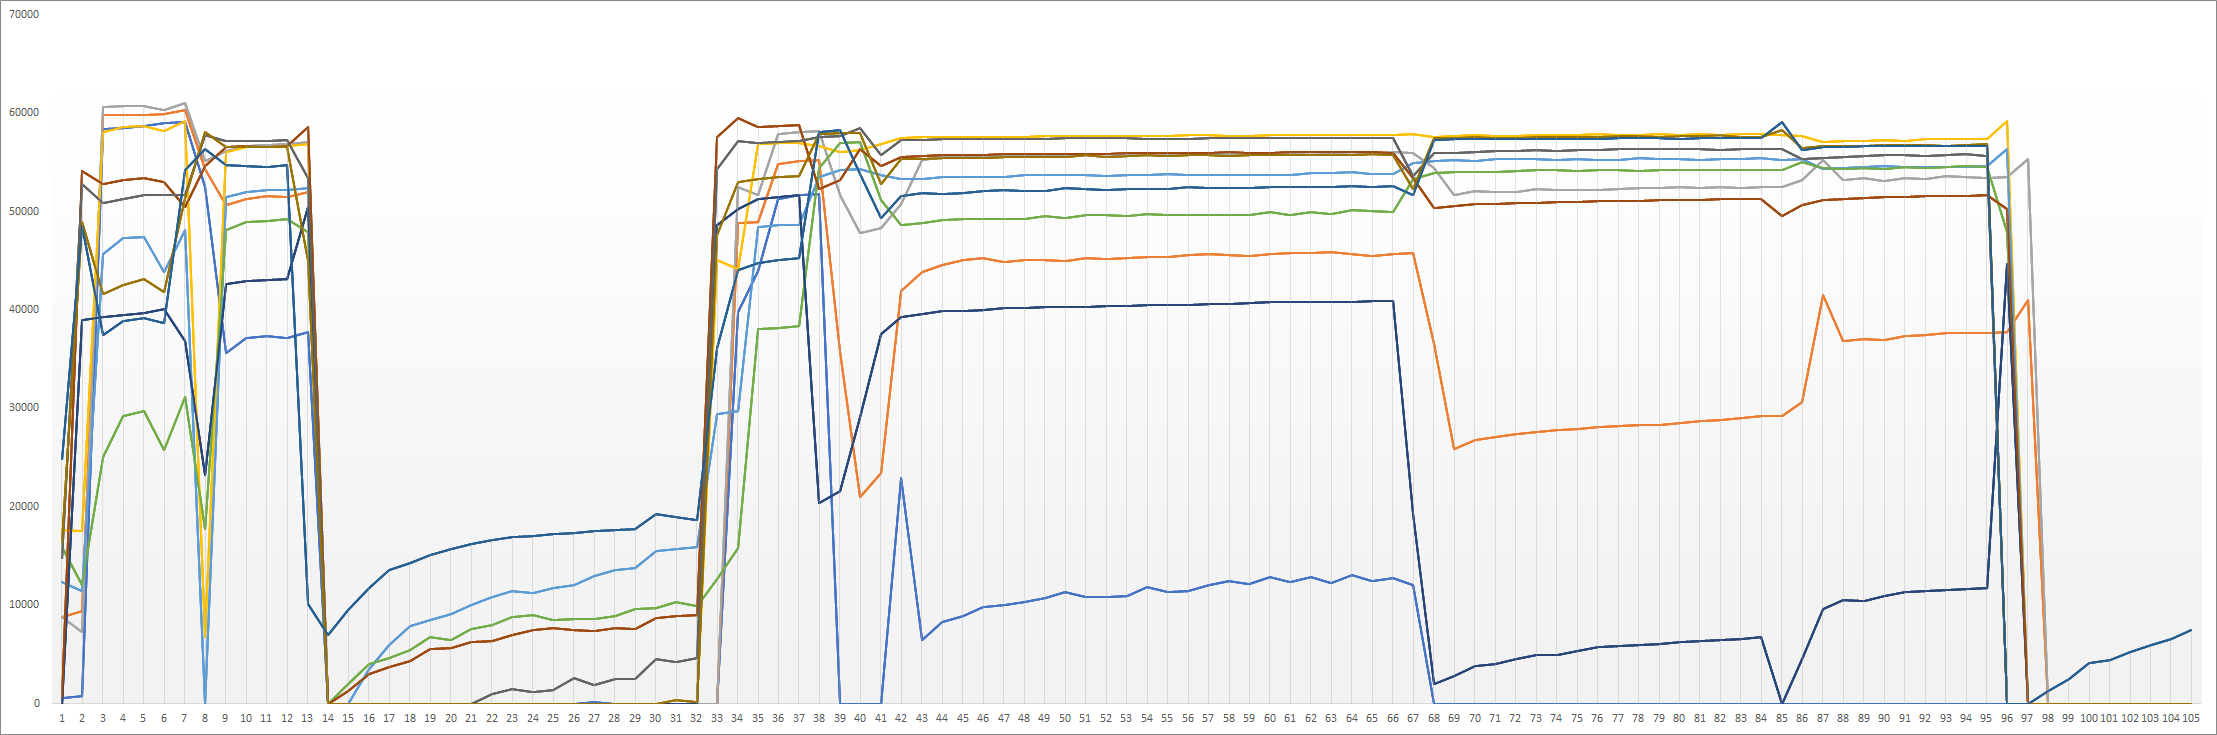
\includegraphics[width=\linewidth]{6-node_2.png}
  \end{center}
  \caption{Pressure measured on sensors in upper torso area.}
  \label{fig:node_2}
\end{figure}

A data from the single sensor, located in the middle of chest area was further analysed. The goal was to see if it is possible to detect breathing. A reoccurring pattern with an interval of 20 seconds was observed. Regular respiratory rate is between 12 and 18 times per minute which should roll out this pattern being breathing. To be able to detect breathing a system sample frequency should be at least double the respiration rate. In case of respiration this means that single sensor sample period should be at least 1.6 seconds. Conducted measurement had sample rate of 4 seconds which means that sample rate should be greatly increased for the future tests.